\documentclass[12pt,aps]{revtex4}
\usepackage{graphicx}
\begin{document}
\title{Decline in trust in modern molecular biology}
\author{Sergey Feranchuk}
\noaffiliation
\email{feranchuk@gmail.com}

\begin{abstract}
BACKGROUND   Some of the priorities which are everywhere in modern molecular biology need to be questioned in the face of the vulnerabilities which are becoming visible due to the recent pandemic. The need to deal with big data, and the need to deal with non-equilibrium systems, are a potential cause of risks and artifacts, even up to illusions of a large scale which have a support in itself. And some of the priorities in molecular biology are indeed just illusions, which means that much of the effort made by microbiologists is made in vain.

METHODS   Illusions cause a decline in reliability, and suggest a change of priorities. To detect and localise some artifacts, tools from information theory and statistical physics were applied to some example cases of molecular biology, both in different subject areas, and of different scales. These artifacts can be classified, either as a convergence to a wrong local minimum, or as a stable illusion supported by positive feedback, just like many of the common causes of malfunctioning in complex systems.  The subject areas under discussion are too complex to suggest true solutions to the problems. But in each of the cases, some hints are provided about the direction to go for recovery from the artifacts.

RESULTS   The subject areas which are discussed as case studies are : - evolution of early humans; - early development of embryos; - prediction of protein structure; - inhibition of tumours; - herbal medicine. In the last of these subject areas, the underestimated value of herbal preparations for the treatment of the coronavirus infection is stressed. And a classification of some medicinal plants is proposed, which may be an approximate response to the corona challenge.

CONCLUDING REMARK  The causes of some artifacts are uncertain, and there is a lack of confidence which prevents molecular biologists from stepping outside their usual directions. But science is a part of society, and problems of science are the problems of society. However, the risks involved when dealing with uncertainties are a different problem.

\end{abstract}

\maketitle

\section{Introduction}

Science, as a method of accumulating approved knowlenge, is a powerful tool and this
has been acknowledged in full in recent times. However, scientific method like any
method is not guaranteed to be free from vulnerabilities. The types of problems in
scientific research which deal with big data are similar to the problems known in
electrical engineering and numerical mathematics. There are two of them :   -
positive feedback which causes numerical instability or noise in electric circuits; 
 - convergence to a local minima, leading to loss of signal or a trivial solution.

These problems can be observed at any scale, from a small laboratory project to a
big community of scientists doing projects in the same subject area.

Warning :   The recent outbreak of coronavirus has raised questions about
reliability and productivity in the modern scientific system, and in particular
within the area of molecular biology. A few case studies are provided below to
demonstrate the two kinds of errors which, it can be supposed, have a damaging
influence on the directions of scientific research and on certain published results.
Some ''tricks'' which are known to engineers who develop electrical systems or solve
numerical problems, have been enough to localise a cause of error in each case.

The case studies are formatted in a uniform ''engineering'' style to stress their
common features and to point out clearly the sources of error.  In this style, some
details which are important only in the individual subject areas, have been omitted.

In each case an alternative viewpoint and a different direction of study is
suggested. Some of these suggestions are controversial, but they might give positive
hints about disputable questions. These proposals are developed further in the Discussion section.
   


\section{Methods}

The scientific publications are carefully reviewed by specialists in the same subject area. If to suppose that the studies have some declinations, the method to localize a reason of controversy should be rooted beyond the scope of each of discussed subjects. 

The statistical physics when it is applied to stochastic and non-equilibrium systems can provide only some tools to manage some common properties of these systems. These tools are far not enough to resolve complications and to propose solutions in the applied problems under study. But negative statements of statistical physics can make sense in a projection to applied problems, just like declaration of the second law of thermodynamics had stop a lot of useless efforts to invent ''perpetuum mobile of the second kind''.

The information theory and the fractal theory did continue a development of this branch of science, providing often not a complete theory but negative statements and heterogeneous but useful tools. The methods in the presented study are based in part on results of modern statistical physics applied to economy, a so-called ''econophysics'', which was presented in series of studies including \cite{CI1}. The model which was described there allowed them to guess the degree of separation between ''rich'' and ''poor'' parts of society, unifying Pareto law and Boltzmann-Gibbs law in a single distribution. In a personal ''portfolio'' of the author is an assessment of some models from microbial ecology \cite{CI2}, where parallels of these systems with a structure of society were discussed.

All of the statistical tools which are used to show the artifacts in cases described below come from the context of these models. The details specific to the each of the subjects are discussed at a qualitative level. 

\section{Results}

\subsection{A case of convergence to a local minimum due to over-simplification}

\emph{Subject} Genomes in the evolution of humans

\emph{Statement under question} Differentiation of genetically modern humans may have started as early as 100-120kyr ago” [3]; ”the genetic separation of non-African ancestors from African Yoruban ancestors started long before 50,000 years ago”[4].

\emph{Method} ”To validate our model, we simulated a hundred 30Mbp sequences with a sharp out-of-Africa bottleneck followed by a population expansion, and inferred population size history with PSMC [pairwise sequentially Markovian coalescent]” [3], ”we propose an alternative approach that we call Multiple Sequential Markovian Coalescent (MSMC), which overcomes the increase in complexity by introducing a different simplification.” ”the MSMC model is a specialisation of the sequentially Markovian coalescent model for the case of two chromosomes. The free parameters of this model include the scaled mutation and recombination rates, and piecewise constant ancestral population sizes. ...”The estimation-maximization iteration started from a constant-sized population history. ”To test the robustness of the model, we introduced variable mutation rates and recombination hotspots in the simulation. The inference is still close to the true history. A uniform rate of SNP (single nucleotide polymorphism) ascertainment errors does not change our qualitative results, either.”

\emph{Controversy} The neutrality model of mutations is implied in the design of the study, but mutations in the human genome do not obey neutrality. Convergence of iterations in the EM approach is not guaranteed if the probability model is wrong, and an illusion of convergence can arise due to the choice of initial approximation. Convergence of the method in simulations which obey the assumed probability model is not evidence that the method will converge in the data which do not obey the model.

\emph{Expanded description}

Genomic data does not fully fit the assumptions about normality and neutrality. The exceptions and deviations from neutrality have multiple causes and dealing with these exceptions and even measuring them, is too complex. However, these exceptions do increase error and disperse the results; they can also cause repeated convergence to a false solution.

Simple tests on simulated data can demonstrate the vulnerabilities of the MSMC method when it is applied to genomes where, anyway, mutation rates do not obey neutrality. The simulations given below are just a few rounds of genome replication. But perturbations from neutrality were introduced in the simulations, assuming that the distribution of mutation rate depends on the position in the simulated ”genome”, and follows a pre-defined rule.

Charts in fig. 1 demonstrate cases when the MSMC approach is unstable. In the control case on fig. 1A), the eight ”genomes” are generated by three rounds of replication. The series of MSMC runs converged there to stable predictions of the expected TMRCA (time since most recent common ancestor), for any mutation rate and for over-dispersed ”genomes”.


\begin{figure}[h]
\flushleft \large \textsf{A}\\
\vskip 4pt
\centerline{\includegraphics[width=\columnwidth]{fig_msmc.png}}%,natwidth=3289,natheight=1497
\flushleft \large \textsf{B}\\
\vskip 4pt
\centerline{\includegraphics[width=\columnwidth]{fig_msmc_diploid.png}}%
\caption{Performance of MSMC in simulations of exponential growth. MSMC runs were adjusted to 4 stages with equal size, with 20 rounds of EM iterations. The estimated beginning of the last stage was treated like a tree-depth. The dependency of tree-depth on the average mutation rate is shown for uniform mutation rates and for the two types of uneven distributions. The tests were repeated 5 times at each point, with different random seeds. In some tests the MSMC runs did not converge; error bars on the upper row were normalised by a chi-square criteria to stress the dependency on the number of successful runs. (A) Control case: eight ”genomes” were generated by 3 rounds of replications. (B) Case of instabilities: another 4 rounds of replications, ’diploid’ genomes were emulated by coupling the simulated ”sequences”.}
\label{fig_msmc}
\end{figure}

In the next series of simulations, eight genomes were generated by four rounds of replication, coupled to ”diploid” sequences. This coupling emulated several variants in some locations of the ”genomes”. And in this case MSMC performed well for a simple test with uniform distribution of mutation rates. But it started to behave unstably in the tests with ”over-dispersed” mutation rates (fig. 1 B).

Time points in the statements are based on the presence of divergencies in the reconstruction of population history for selected ethnic groups, in contrast to the convrgence of population histories at very early times. But the presence of distortions in the method can introduce perturbations in the results. These perturbations are accumulated back in the time scale due to the iterative nature of the method. So the time points in the concluding statements can be declared to be much earlier in the past than they should be.

\emph{A suggested viewpoint to the subject}

Straightforward distance-based methods of phylogeny are poorly supported by any probability model. They are direct rather than iterative, and they have linear dependency on perturbations in the input data, unlike probability-based methods which, in the worst cases, have exponential instability. 

\subsection{A case of positive feedback due to over-complication}

\emph{Subject} Development of embryo by methods of RNA-seq

\emph{Statement under question}  ''development [of embryo] comprises the coupling of early and late phases of conserved gene expression. These phases are linked by a divergent 'mid-developmental transition' that uses species-specific suites of signalling pathways and transcription factors'' [''reversed bottleneck'' model of evolution]. ''this transition are crucial for defining the phyletic body plan '' \cite{CR2}.

\emph{Method} ''we compare the developmental transcriptomes of ten species, each annotated to a different phylum, with a wide range of life histories and embryonic forms'' \cite{CR2}. ''To establish the direction of the ordered samples, we show that an appropriate indicator is the entropy of transcriptomic gene expression levels, which increases over developmental time'' \cite{CR1}.

\emph{Controversy} Some common rules and features are observed in chaotic and nearly chaotic systems, like an appearance of  fractal dimension or ''intermittency''. The development of embryo as any early development is unequilibrated and exceed of over-dispersion here can lead to some rules which seem to be common in all range of similar systems. But these rules are just artifacts of statistical distributions, it can't be used to derive long-coming consequences. The declared association of the observed effect with evolution of species are not supported with any valuable evidences besides an approximate match in a positioning of the comparable events on relative time scales.

\emph{Expanded description}

Some part of genes in any cell are expressed in large quantities, some are expressed only in particular phases, and some are expressed at moderate level. The profile of gene expression sorted following an abundances in usually a combination of power-law distribution for highly expressed genes and exponential distribution for moderately expressed genes. This is just a statistical property of a complex system of that scale. The moderately expressed genes provide a wide spectrum of background and support for an activity of the cell but their distribution itself says nothing about any specifics of their activity. 

Another generic statistical property of that systems is that in a course of intensive development the fraction of 'power-law' (Pareto) part of the distribution becomes lesser. This property has the same meaning as the declared in \cite{CR1} observation that entropy of gene expression profile is increase with development time. 

These two generic properties are enough to explain an appearance of ''phase transition'' in a comparison of two similar systems, of any kind. These systems can be almost identical, as in fig 2A or, simply just be of the same class as the two unrelated texts in fig 2B. In the development of any system the key ''players'' within it are changing, whether it is a system of genes or a lexicon of a text. If the two systems are of the same class, the players in it will anyway have something in common. And when the key players are independently changing in both systems, a correlation between the comparable stages of development will anyway change and even have a 'bottleneck'' like in fig. \ref{development}A, simply because the profiles of abundances in both systems are changing according to the same generic rule.

The absolute value of the ''bottleneck'' effect in the artificial example in fig. \ref{development}A is much less than was observed for the development of embryos. But this example demonstrates that an appearance of the bottleneck effect is just a trivial consequence of the method in which the comparison of the systems is presented. And it is trivial that any pair of species will have something in common; they both have systems of gene regulation. So the described effect, in fact says nothing additional to what is already known about the embryo development of each of the considered species. The effect itself appears just because of the profiles in the two systems are changing according to the same rule. And the reordering of the samples in the preliminary stage of the pipeline put the profiles of genes in the order which is most appropriate to observe the effect; i.e. the effect is amplified.

\begin{figure}[h]
\centerline{\includegraphics[width=0.95\columnwidth]{development.png}}
\caption{Artificial correlation maps which illustrate the explanations of ''reversed bottleneck'' effect.
(A) Distributions which simulate profiles of gene expression with increasing fraction of ''exponential'' part.
(B) Distributions of common meaningful words the two unrelated scientific publications, which illustrate a presence of commong features in dveloping narratives. Profiles of ''expression'' at each of seven stages are shown in the left of both maps in log-log coordinates. Texts of the studies \cite{CE2} and \cite{CR2} were used for a comparison of narratives.
}
\label{development}
\end{figure}

\emph{A suggested viewpoint to the subject}

The development of human and closely related species is investigated much more thoroughly than a development of distant phyla. A grouping of gene system into pathways and subsystems is the only way to get some outcome from an analysis of gene expression. A neutral grouping of genes by methods of subcommunity detection should be considered in the analysis of gene regulation in distant phyla, without a need to rely on homologs and parallels in other lineages.

\subsection{A situation of convergence due to over-simplification}

\emph{Subject} Prediction of protein structure

\emph{Statement under question} ''CASP (critical assessment of structure prediction) assesses the state of the art in modeling protein structure from amino acid sequence. The most recent experiment (CASP13 held in 2018) saw dramatic progress in structure modeling without use of structural templates'' \cite{CC1} ''Despite not explicitly using template information, the results [of Alpha-fold system] in the template category were comparable to the best performing template-based methods'' \cite{CC2}

\emph{Method} ''CASP ... is a biennial community experiment to determine the state of the art in modeling protein structure. Participants are provided with amino acid sequences of target proteins, and build models of the corresponding three‐dimensional structures. Submissions are compared with experiment by independent assessors. The experiment is double blinded—participants have no access to the experimental structures and assessors do not know the identity of those making the submissions.'' ''A neural network  trained to predict the distances between the β‐carbon atoms of pairs of residues. Contact prediction has been extensively used in structure prediction but previous work has also made residue distance predictions ... These distance distributions are modeled with a softmax distribution for distances in the range 2 to 22 Å split into 64 equal bins. The network is trained to predict distances between two 64‐-residue fragments of a chain, giving a probabilistic estimate of a 64 x 64 region of the distance map''

\emph{Controversy} The target structures which are provided on each round of CASP are selected to avoid similarity with common structures of proteins, and respectively to results of previous rounds. Inter-residue distances are now used extensively in structure predictions. The successes of these methods in previous rounds have been echoed in the average complexity in the distribution of inter-residue distances for CASP targets. It has become lower than for randomly selected protein structures. This means that software, which relies on inter-residue distances and performs well in CASP, will perform poorly in general-purpose structure prediction.

\emph{Expanded description}

The CASP project was established in 1994. The project was set up as an experiment which was intended to assess the abilities of scientific groups to predict the 3D-structure of proteins from their sequences.

13 rounds of the ”experiment” have occurred since 1994; the latest complete round was in 2018. Several dozens of ”targets” have been presented in each round; these targets were usually the sequences of proteins for which the structure had already been determined but for which free access had been postponed.

The reduction of a protein structure to its contact map was the most promising approach in early attempts of ”template-free” structure prediction. By following this approach, it became recognised that to represent a contact between residues as a binary value was not efficient enough and a more precise representation of the distance between closely located residues was required. This idea came to prevail, and in the approach [8], which won the latest round of CASP, distances between residues were split into 64 bins.

The problem of protein structure prediction is hard to solve and the folds of proteins are complex. The estimates of complexity of the CASP targets which are shown in 3 illustrate the presence of hidden simplicity in the averaged properties of these targets. Therefore, in following rounds, the structures of the targets can be be predicted more easily, if reliance is placed on this simplicity.

The values of entropy in fig 3 are obtained using the different ways in which a protein fold can be reduced to a set of binary distributions, that is: square fragments of a contact map (1), hashed distances in triangles (2), hashed distances between C$\alpha$ atoms (3), four hashed distances between C$\beta$ atoms in the nodes of a square at contact map (4).

Some decrease in the entropy of the distance-based metrices 3 and 4 can be observed in fig. 3A. in the targets from CASP rounds 2 to 4. After several rounds of CASP, the idea of reconstruction of distance maps proved to be most efficient; the performance of these best approaches could have influenced the strategy by which targets for next round were chosen.
The value of entropy is the minimal quantity of information which encodes the complexity of a distribution. But the measure of complexity which can assess the difference between CASP targets and other structures is the information value found in the common code of PDP templates, not in the code of the structure itself. This value should be a bit greater than the conventional entropy. In the case of the brief analysis provided, it is expressed as $\sum{p\log{p_0}}$; where $p_0$ is the probability of a bin in a distribution, averaged through structures in PDB. So the distributions of entropy are shown on fig. 3B, together with the updated information values, at a scale adjusted to the average entropy of PDB structures.


\begin{figure}[h]
\flushleft \large \textsf{A}\\
\vskip 4pt
\centerline{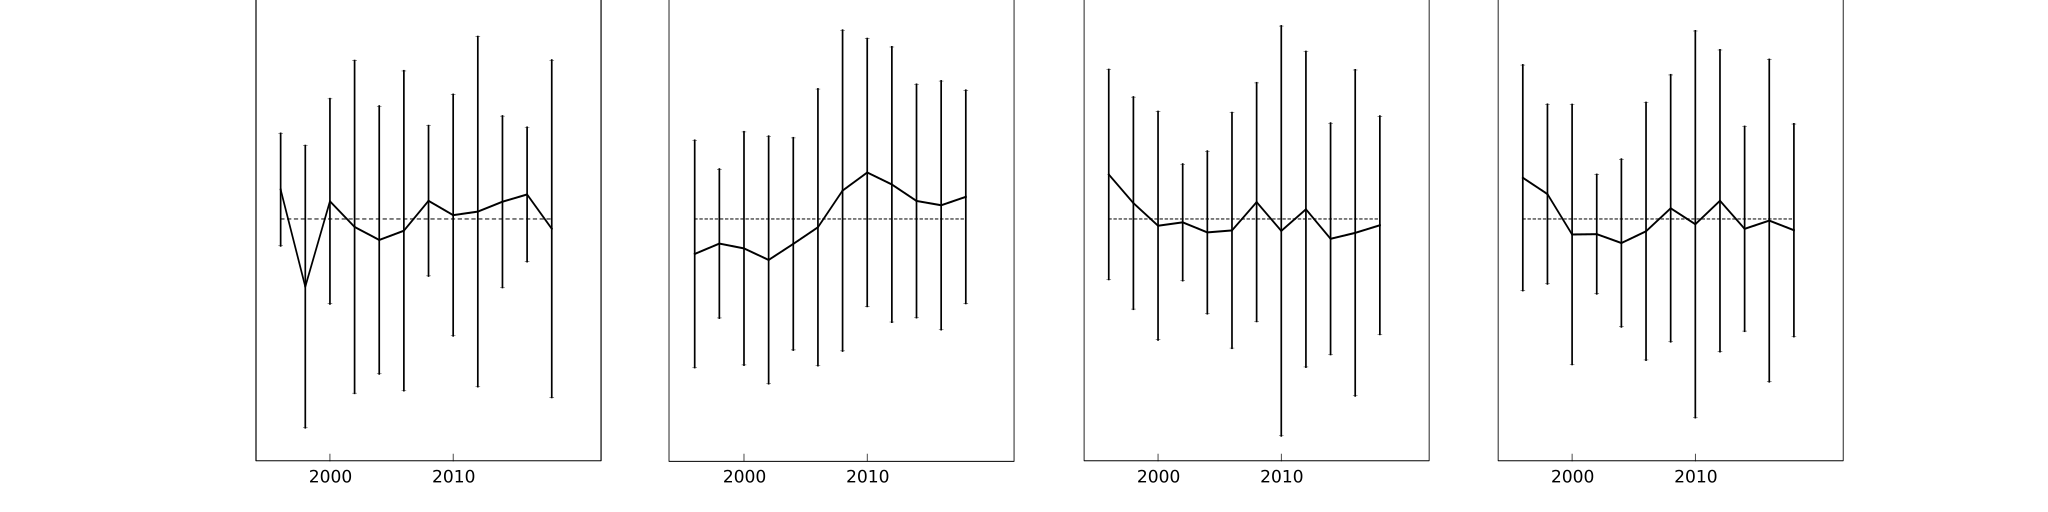
\includegraphics[width=0.85\columnwidth]{casp_f1.png}}
\flushleft \large \textsf{B}\\
\vskip 4pt
\centerline{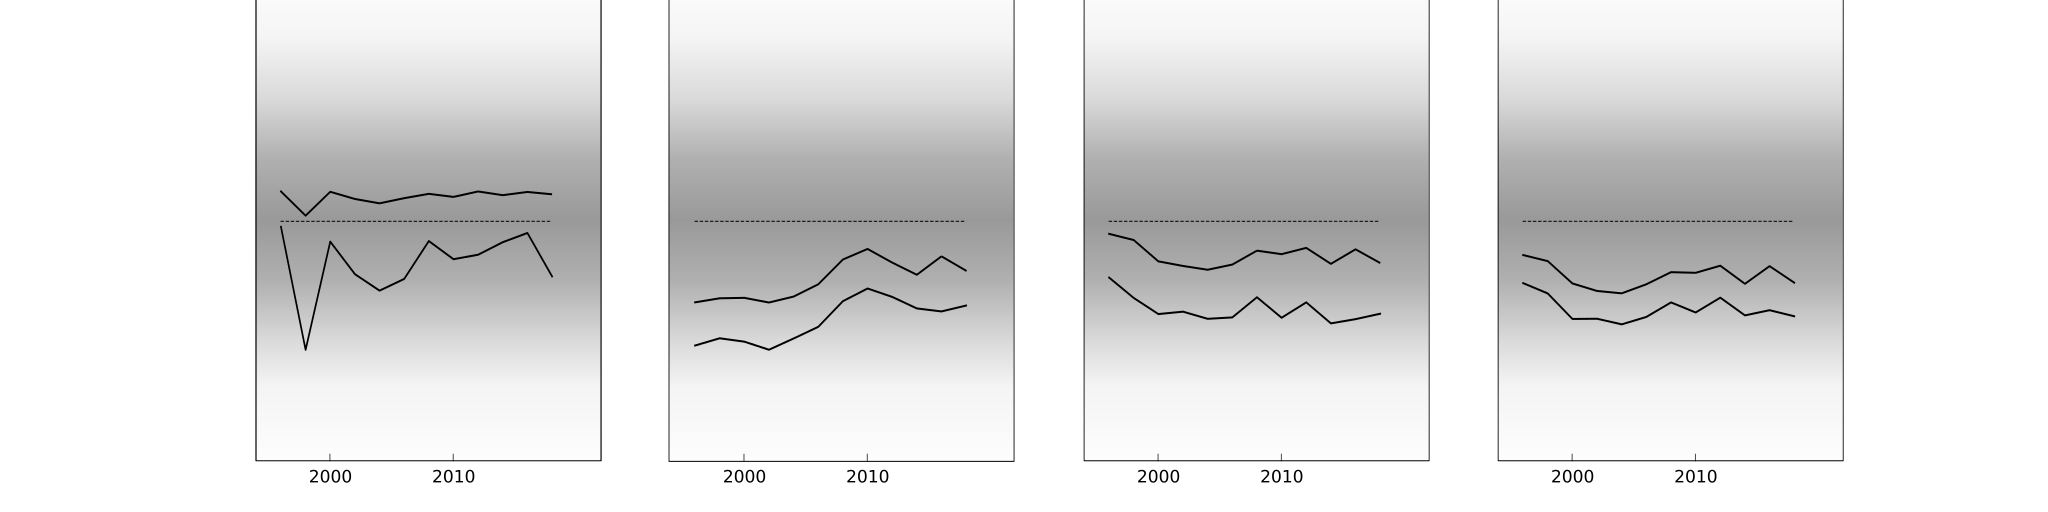
\includegraphics[width=0.85\columnwidth]{casp_f2.png}}
\caption{(A) Distribution of entropy measures for the targets of 11 rounds of CASP. Error bars are adjusted to standard deviation (SD) of the measure in each round. Margins in the charts are adjusted to 2 SD from the average across all targets. Labels on the X axis are the years of the competitions. (B) Distribution of entropy measures (solid line) and of the relative information values (dash-and-dot line), are for the targets of CASP. Margins are adjusted to 2 SD from average in PDB; and a shadow gradient in the background shows Gaussian distribution around that average. }
\label{casp_f12}
\end{figure}

The distance-based metrics for CASP targets are lower than average in PDB, and no correction was made for this bias. So, by metric 4, of the two distance-based metrics, the relative entropy is closest to the true entropy. This means that, for the case of CASP targets, the methods which were trained on templates from PDB by similar metrices will guess the template structures in a new round of CASP more successfully – with an increased gap in their ability to predict neutrally selected protein structures.

\emph{A suggested viewpoint to the subject}

The hierarchical organisation of protein structures and the repetitive presence of common structural motifs suggest that the problem of direct evaluation of entropy of protein folds can be reduced by splitting it into sub-problems. Local sub-chains of the structure could have their flexibility measured separately. Such sub-problems are solvable in reasonable computation times. What’s more, the ability to manage with only the entropy terms in a protein's energy balance, would open the way to the prediction of protein structures from physical principles without the need to rely on any of the statistical properties of known folds.  

It is hypothesised that the genome contains a group of genes which can cause the brain to send a signal which induces a tumour elsewhere in the body. This group of genes evolved for other purposes and other situations. Unfortunately, they have been conserved by evolution, despite the damaging effects when they are activated. 

\subsection{A situation of positive feedback due to over-complication}

\emph{Subject} Discovery of cure for cancer.

\emph{Statement under question} ''Carcinogenesis is a multistep process attributable to both gain-of-function mutations in oncogenes and loss-of-function mutations in tumor suppressor genes. ... In recent years, several promising strategies directed at tumor suppressor genes, or the pathways controlled by these genes'' \cite{CO1}

\emph{Method} ''Historically, the idea that cancer could be etiologically attributed to genetic alterations was first recognized when cancer-causing viruses were found to be able to transform normal cells.'' \cite{CO1} Since the idea about genetic origins of cancer was accepted, the efforts of research groups were focused on how to inhibit in some way the activity of some oncogenes and/or to enhance in some way the activity of tumor suppressor gene.

\emph{Controversy} An ability to treat of cancer is important medical challenge and research groups who tried to solve this challenge get priority funding. A gene regulation in any cell is complex and being focused on some particular gene and having enough funding a lot of new results can be discovered. These results raise the hopes that the selected gene is promising to be important for a treatment of cancer, and increase the hopes to an initial hypothesis about genesis of cancer. This process is self-consistent and do not depend from an initial hypothesis and on selection of candidate genes; promises and hopes to get a treatment for cancer in a result become an illusion. 

\emph{Expanded description}

The treatment of cancer is an important subject of molecular biology and is developing extensively. And science, in common with the rest of society, has both  ''rich'' and  ''poor'' subjects to be investigated. The treatment of cancer is certainly a ''rich'' subject. Many scientific groups are focused on the study of some particular gene or genes, which are classified as oncogenes or as tumour suppressor genes.  

Within a model of ''econophysics'', the assets of ''rich'' society are distributed following a Pareto law, while the assets of ''poor'' society are distributed following an exponential law. So, the degree of interest in specific subjects related to oncology can be expected to be distributed according to a Pareto law. But confirmation for this hypothesis still needs to be provided. One straightforward approach to get this confirmation is the text-mining of biomedical literature,

Science is not a society, and scientific disciplines are not separated obviously and distinctly. The best that can be expected is an estimation of the measure of interest to some subsample of clearly defined disciplines. A convenient way to do this is to count the number of publications in which oncogenes are mentioned.  Two sets of nearly randomly selected oncogenes were used to compare the fit of publication activity to Pareto and to exponential distributions, as it is shown in fig. \ref{oncology_pareto} A. Herbal medicine is a ''poor'' direction of science where exponential distribution of terms is expected, and the results for two subsets of generic Latin names of medicinal plants are show in fig. \ref{oncology_pareto} B as control cases.

\begin{figure}[h]
\flushleft \large \textsf{A}\\
\vskip 6pt
\centerline{\includegraphics[width=\columnwidth]{oncogenes_pareto.png}}
\flushleft \large \textsf{B}\\
\vskip 6pt
\centerline{\includegraphics[width=\columnwidth]{herbal_pareto.png}}
\caption{Compares the entropy measures for the selected subsets of keywords for which counts of publication in Pubmed and PMC databanks were obtained. The size of the dark bar shows the measure of fitness to a Pareto distribution, and the size of the light bar shows the measure of fitness to an exponential distribution. 
}
\label{oncology_pareto}
\end{figure}

The contrast between the two disciplines of scientific studies is clearly seen in the results presented in fig. \ref{oncology_pareto}. The genes considered as oncogenes or tumor suppressors are mentioned much more frequently in the scientific publications than the names of medicinal plants, both in abstracts and in the main text. And these frequencies, with minor exceptions, are better described by a Pareto distribution in the case of oncology studies and by an exponential distribution in the case of herbal medicine.    

Pareto distributions are characteristic of societies in which there is competition. Winners of the competition rise to the top of societies, and their incomes increase due to the properties of commercial brand names and financial assets.
But science is not a society, and the rules of science are in some way opposed to the rules of society. The efforts of scientists are supposed to be done with collaboration and cooperation !

\emph{A suggested viewpoint to the subject}

It is hypothesised that the genome contains a group of genes which can cause the brain to send a signal which induces a tumour elsewhere in the body. This group of genes evolved for other purposes and other situations. And they have been anyway conserved by evolution, despite the damaging effects when they are activated.

\subsection{Another situation of convergence due to over-simplification}

\emph{Subject} Herbal medicine

\emph{Statement under question} ''The media has reported that some people are seeking ''alternative'' remedies to prevent infection with COVID-19 or to treat the virus. Some of these purported remedies include herbal therapies and teas. There is no scientific evidence that any of these alternative remedies can prevent or cure the illness caused by COVID-19. In fact, some of them may not be safe to consume.'' ''Globally, there has
been an increase in the use of herbal remedies including traditional
Chinese medicine (TCM). ...a multidisciplinary approach to assessing
the molecular content of 26 TCMs ... showed 92\% of the TCMs examined
were found to have some form of contamination and/or substitution.''
[10] (https://www.nccih.nih.gov/health/in-the-news-coronavirus-and-alternative-treatments)

\emph{Controversy} The composition and effect of medicinal plants is complex
and a lot of effort is required to keep scientific support for herbal
medicine at a proper level. The gap between the demand for these
efforts and the funding of this approach has led to a need to rely on
''traditional'' controversial opinions. These controversies lead to new
disappointments and to an increase in the gap.
 
\emph{Expanded description}

The active compounds of medicinal plants oppose pathogenic communities
which damage the plants’ development. They are often specific to
climate and geographical region. The damage caused by pathogens can be
reduced either by direct inhibition, or by correcting the balance in
the microbial community; the composition of active compounds in plants
is often targeted to the second strategy.

The diseases of human are often directly or indirectly caused by
pathogens rather than by damages in the genome or other internal
problems. The composition of the pathogenic communities which attack
humans have much in common with the communities which attack plants in
the same region. Therefore, herbal preparations can be effective in
the treatment of many diseases. However, the strategy of correcting
the balance of microbial communities has the risk of misuse and
adverse effects. Microbial balance can be moved in the wrong
direction, if herbal prescriptions are used improperly.

Herbal preparations are known to be effective as medicine in most
cultural traditions. Modern herbal medicine makes use of this
knowledge, but it sometimes leads to misunderstandings and
disagreements between scientific approaches, even within herbal
medicine itself. Opinions here are even more diverse now, than in
times when most of medicine was based on the ”traditions” of local
cultures (fig \ref{herbal_geo}).

\begin{figure}[h]
\centerline{\includegraphics[width=0.8\columnwidth]{fig_herbal.png}}
\caption{Left: clustering dendrogramms for (A) interests of scientists from
different regions in recent publications on herbal medicine, (B)
traditions of herbal medicine, reconstructed from the extensive list
of psychoactive drugs, as it was published in [11]. Size of bars are
for 50\% correlation between publications on different plants (A) and
for 50\% of commonly known plants (B). Right (C): PCA chart for
traditions of origins for medicinal plants in modern herbal medicine.
Sizes of circles reflect total counts of references to a region. The
detailed description of the presented analysis is in the supplement
text.
}
\label{herbal_geo}
\end{figure}


When knowledge is incomplete and demand is high then cases of misuse
are almost inevitable. These cases lead to the growth of
disappointment in a whole spectrum of these methods. If you look at
herbal medicine from the outside, this is completely natural. Thus,
the important and valuable abilities, and the potential power of
herbal preparations have become almost ignored.

\emph{A proposal for positive solution}

The use of accumulated data on genomics and a gene regulation is a
neutral way to approximately assess herbal preparations, and to help
to choose between them.
There a long list of medicinal plants and their usefulness can be
approximated by matching their expected effects to cases of specific
medical disorders. If the prescribed treatment needs a combination of
several plants, this can be approximated by dividing the expected
effects of a plant into three directions, towards relaxing of
direct damages of disease, towards strengthening of internal defence, and
towards stabilisation of side effects.

Diseases of humans can be associated with medicinal plants at the
level of gene regulation, if the profile of gene regulation for the
disease is known from RNA-seq experiments.

Difference between profiles of expression was estimated using
fragments of expression profiles for pre-defined subsets of loosely
related genes, separated into clusters. In each of RNA-seq experimentd
the samples from both diseased and control gropud fall into one of
several clusters.

Three additional scores were estimated in this setup: (1) ''removing
positive symptoms'' - cluster of profiles which was abundant in
diseased state should become less; (2) ''removing negative symptoms''
- cluster of gene states which is abundant in healthy state should
become bigger; (3) ''removing risk of side complications'' - clusters
of gene states which are not abundant in healthy state should not
become bigger.        


Diseases of human can be associated with medicinal plants at a level of gene regulation, if a profile of gene regulation is known for a disease, and it was obtained from available RNA-seq experiments. The direction of gene regulation caused by medicinal plant was
extracted from biomedical publications, and medicinal plants are distributed there from too popular to rare and underestimated. For extensively studied plants more is known to assign a high score of the expected effect. The ordering of an expected effect from popular plants down to rare plants is looking like it is shown in fig.  \ref{fig_herbal_positive} A.  

In the case of coronavirus infection, the estimates of effects of
medicinal plants which are shown in fig \ref{fig_herbal_positive} B are not supported by clinical
trials or any sequencing data, but are obtained by extrapolation from
other experiments. The characteristics of the coronavirus infection
are the following: (1) it is a virus infection. (2) it causes
inflammation in the lower respiratory tract. (3) it often causes
diarrhea. (4) the course of disease is often complicated by damage
from other opportunistic pathogens in lungs. So, four RNA-seq
experiments were combined in the extrapolation: cells of inflamed
lungs in asthma; liver cells infected by HCV; inflamed cells in
ulcerative colitis; blood cells of those who are vulnerable to
tuberculosis.



\begin{figure}[h]
\centerline{\includegraphics[width=0.95\columnwidth]{fig_herbal_positive.png}}
\caption{
(A) Rank-abundance distributions of scores with expected effect of
medicinal plants in cases of processed profiles of diseases. (B)
Ternary diagram for a case of lung inflammation due to virus
infection. Sizes of the circles show the values of the expected
effect, which have been transformed from probabilities by quantile
normalization.}
\label{fig_herbal_positive}
\end{figure}

Several common and well known plants were selected to be shown in
chart  \ref{fig_herbal_positive} B, to show the estimated directions of their activity.  Most of the reported features of medicinal plants are
known, the direction of their effect is expected and the extent of
their safety is documented. From these plants, Echinacea and Rhodiola,
which are classified as stimulants and adaptogens, direct their effect
towards reducing negative symptoms and side complications. Onion or
garlic, from the genus Allium, as well as some other preparations,
(e.g. core of oak), are mostly directed towards stabilisation against
side complications. Mint and conifers, which are known for their
ability to improve breathing, mostly support the weakness of lungs as
negative symptoms of the disease. Pontentilla, which is known for its
anti-inflammatory and anti-diarrhea effect is probably acting more
directly to soften the damages caused by the increased pathogen load. Coriander,
marticaria (chamomile) and passiflora for which an anti-inflammatory
activity has been observed are also expected to be directed in part
towards reducing the positive symptoms of the disease.

Of course, the final decision about a prescription in a case of
infection should be left to a physician. But in a situation of high
risk, the prescription of properly chosen medicinal plants is expected
to usefully soften the damage and complications caused by this
disease. The results described above are only approximate. However,
they should be useful for drawing physicians’ attention back to these
methods of treatment.

\section{Discussion}

\subsection{Evolution of humans}

A straightforward UPGMA clustering is not sensitive to over-dispersion which is a
cause of instability in EM-based methods. The UPGMA tree for human evolution
suggests that ancestors of most of the African population were expanding into other
parts of Africa in the same period as the ancestors of other tribes were expanding
into Eurasia. Some lineages which separated much earlier are present in the genomes
of the African population in minor fractions.

Most of the phylogeny methods strongly rely on a value of mutation rate. This rate
has been observed to change in the course of human evolution, but the direction and
reasons of this change is a cause of confusion. A simple update of the UPGMA
algorithm allows the variations of mutation rates to be estimated, as shown in fig.
7B.

\begin{figure}[h]
\centerline{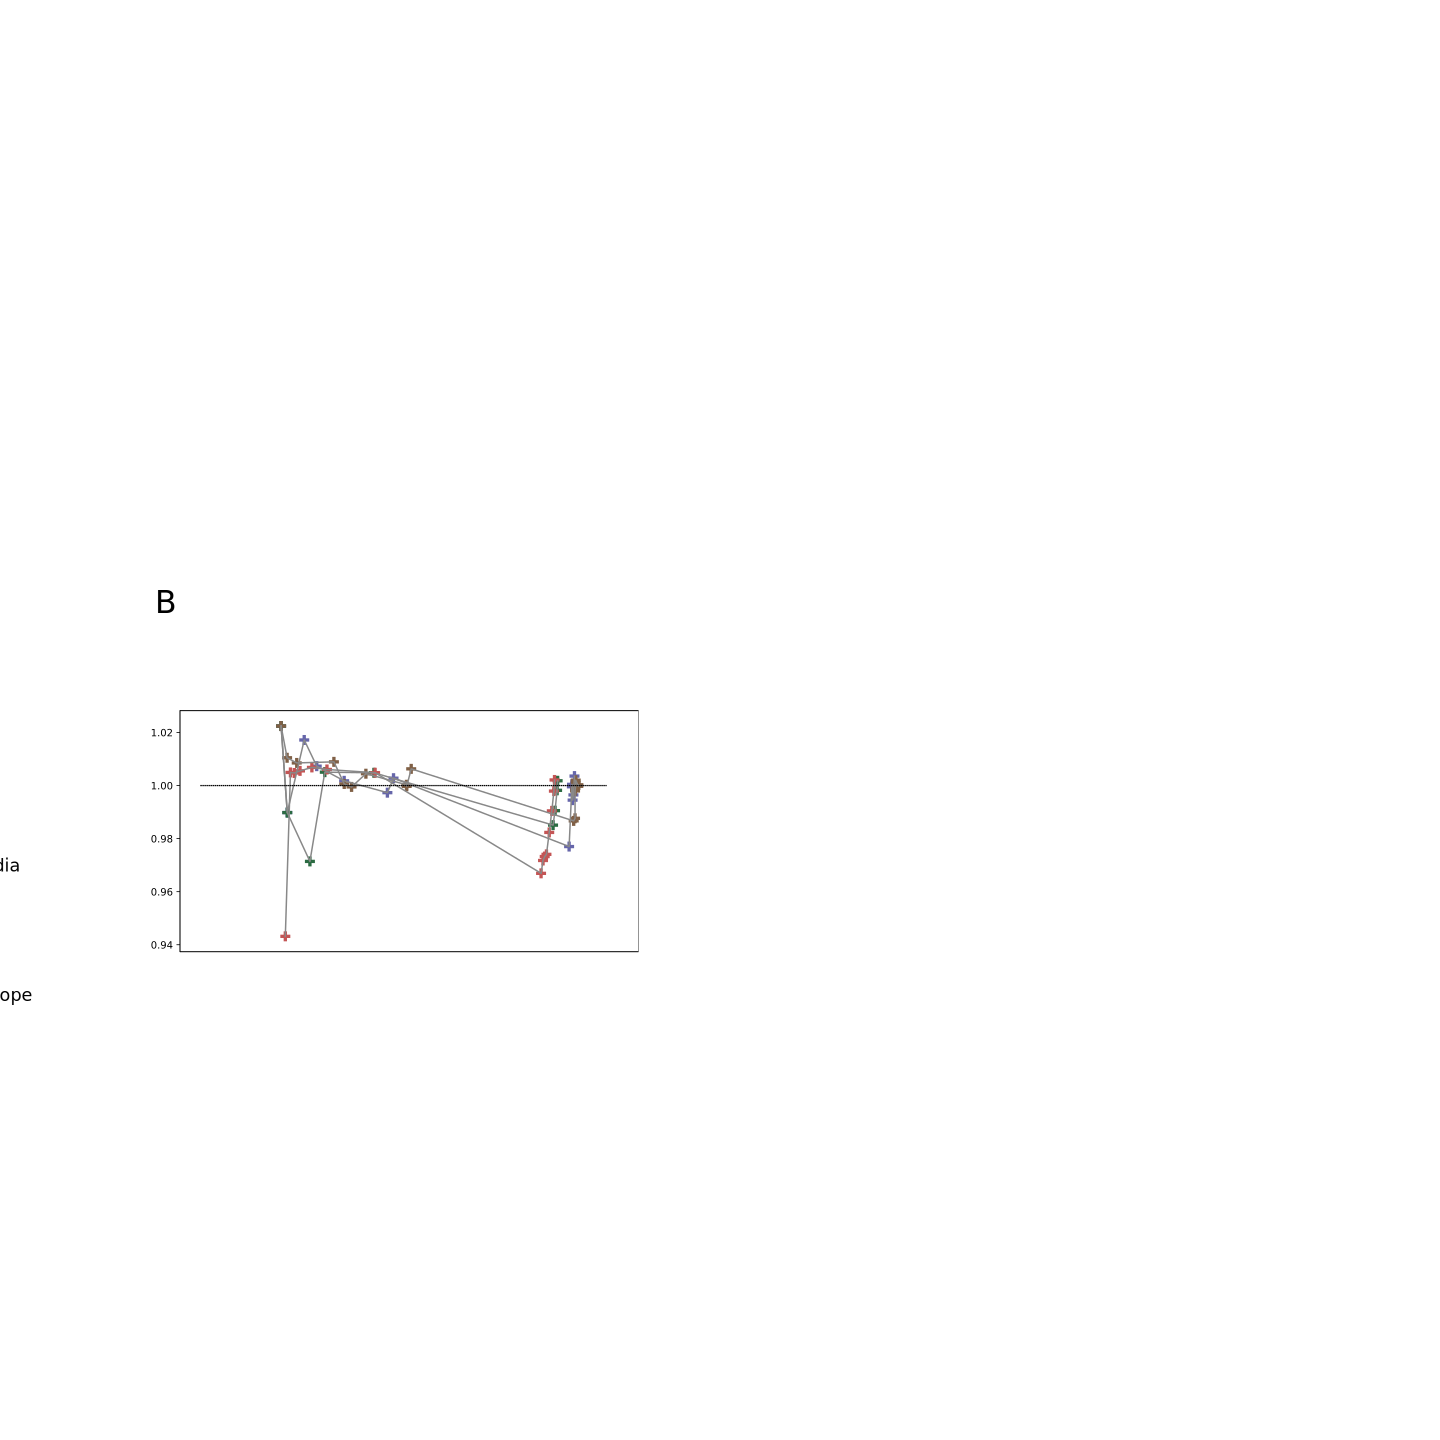
\includegraphics[width=0.95\columnwidth]{fig_evol.png}}%,natwidth=2055,natheight=1237
\caption{(A) Distance-based tree for genomic data from the ”1000 genomes” project,
for selected individuals from several races. (B) Variations of mutation rates in the
course of human evolution, estimated by iterative updating of branch lengths in the
UPGMA tree. The four lines show variations for the four races.}
\label{fig_evol}
\end{figure}

These results indicate that the rate of change was more fast in the times when migrations began.
Then during the period of migrations the rate was decelerated. After these times, around
several thousands years ago, the rate becomes to accelerate. This can be easily
explained. The early humans were developed in a direction of spreading and separation. But when
the Earth became populated enough there was a pivotal point at which the direction
of human adaptation changed towards joining and communication.

\subsection{RNA-seq analysis}

Finding a way to compare embryo development in very heterogeneous species is
difficult. It seems worthwhile to reorder the samples, by the method which in fact lead to an artifact. In the case of model sponge \textit{Amphimedon quennslandica}, it has 6 visually distinguishable
stages of embryo development, from single cell to free-swimming larvae. These stages
are not easily separated by overall gene expression. The stages of other phyla are
not the same as for \textit{A.queenslandica} and they vary from phyla to phyla. Little is
known about gene regulation in some of the species, and the advantage of the
proposed reordering is that it does not rely on any annotation of known genes.

\begin{figure}[h]
\centerline{\includegraphics[width=\columnwidth]{expression_pca.png}}
\caption{PCA decomposition of correlation matrix between samples at three stages of \textit{A.queenslanica} embryo development, for overall gene profiles (A) and for profiles within selected grouos of genes (B,C), for three independent series of RNA-seq experiments were the stages of embryo development were investigated.}
\label{expression_pca}
\end{figure}

But if profiles of expression are limited to some narrow group of genes, as shown in
fig. \ref{expression_pca}, it becomes much easier to distinguish stages of development directly from the
expression data. There is no need to guess the order of a sample, thus avoiding an
approach which tends to be looped to itself.
And pre-defined groups of genes, like a family of similar transcription
factors, fit less than some of the groups selected without being in accordance
with the experiments under study.  And so, in the case of \textit{A.queenslandica}, these
results show a possibility of detailed and specific analysis of
embryo development, without use of any annotation of known genes.

\subsection{Protein structure prediction}

The enthalpy and entropy of folded proteins are delicately balanced towards the
stabilization of a structure. So it can be to assumed that
reconstruction of protein structure from physical principles is impossible, because
direct estimates of entropy are computationally too costly. In this case the only possible approach to guess a target structure is to rely on associations with known protein structures using reduced representations of their folds. 

But it has been observed that an estimate of the entropies of loops between
beta-hairpins can be used to discover the correct ordering of beta-hairpins for
structures of the type shown on fig. \ref{fig_folding}A. So for the case of beta-sandwich proteins,
the problem of finding correct folds can be solved by enumeration of the possible
orderings in which beta-hairpins can fold into a ''sandwich''.

\begin{figure}[h]
\centerline{\includegraphics[width=0.95\columnwidth]{fig_folding.png}}
\caption{(A) In the two proteins of the same ''beta-sandwich'' fold, with PDB IDs 3d33
and 5bxd, the ordering of beta-hairpins is different. (B) Multiplicity of pathways
in an assembly of beta-hairpins, for the case of 3d33 protein.}
\label{fig_folding}
\end{figure}

This idea can be expanded to a generic method for structure prediction. The common
structural motifs of types other than beta-hairpins are used there as ''building
blocks''. There are multiple paths in which assembled substructures can be combined
(fig. \ref{fig_folding}B); this multiplicity reflects the computational complexity of the protein
folding problem. But this computational complexity is reduced to a polynomial by the
use of a hierchical principle. That is, only adjacent segments of chains are allowed
to be joined into a single substructure of the next level in a hierarchy. One or
several best substuctures should then be selected from all possible combinations to
continue the assembly to the next levels.

\subsection{Oncology and neural activity}

If one assumes that the attempts to suppress the activity of oncogenes in causing
tumours are movements in the wrong direction, then some other direction in the
search for a treatment for cancer needs to be suggested. And any such hypothesis
should include something to resolve the ''irrationality'' of oncogenes in the genome.

The hypothesis about a ''neural'' origin for cancer is provided here as an attempt to
resolve this paradox from the other side. The case of sponges in Baikal is a case
where a rational need for oncogenes can be shown. The development of the Baikal
sponge crisis shows that contamination by opportunistic pathogens causes inevitable
death of a whole sponge. And, in the sponge’s symbiotic green algae, there are signs
of adaptation at an extremely high rate (fig. \ref{fig_algae}A). Mutations with such a high rate
are incompatible with most life (in this case the metabolic relations between
symbionts and sponges).

\begin{figure}[h]
\flushleft \large \textsf{A}\\
\vskip 6pt
\centerline{\includegraphics[width=0.8\columnwidth]{algae_mutations.png}}
\flushleft \large \textsf{B}\\
\vskip 6pt
\centerline{\includegraphics[width=0.95\columnwidth]{algae_interpretation.png}}
\caption{(A) The relative proportion of polymorphic sites in a chloroplast genome of
sponge symbiont. (B) Qualitatively assessed abundances of chloroplast substrains in
three samples of sponge. Here, ''2-nd dominant strain'' can be a group which began to evolve intensively when a disease began do develop.}
\label{fig_algae}
\end{figure}

In (https://f1000research.com/articles/7-1405/v2) it is suggested that the
symbiont-genome includes some ''machinery'' which induces such rapid mutations in an
almost desperate attempt to escape inevitable death (fig. \ref{fig_algae}B). And that this
genetic machinery has been conserved in the genome because it has allowed the
symbiont to survive previous crises which have happened in the course of algae
evolution.

The estimated rate of mutations in the symbionts of diseased sponges is comparable
to the rate of mutation in some tumours. Therefore, if the onset of rapid adaptive
mutations in algae is ''rational'' in the case of a deadly disease of its host, then
perhaps the onset of a tumour in humans also has a certain ''rationality''. If so,
this should originate in the CNS (Central Nervous System) since this is the origin
of most other processes in the human body. And some associations between tumours and CNS are anyway become to be detected in trends of modern scientific research (fig. \ref{fig_adaptive}A). 

\begin{figure}[h]
\centerline{\includegraphics[width=0.95\columnwidth]{oncology_neural.png}}
\caption{(A) Shows the number of publications in Pubmed per year, for the specified
terms combined with the terms ''Cancer'' or ''Tumour’'. (B) Mean-difference chart for
genes related to apoptosis. From these genes, the genes annotated as facilitating
apoptosis are shown as squares. Y axis - average expression level, in number of
reads aligned to a gene, X axis - increase of expression level (''fold count'')
relatively to a control group. Both axes are in logarithmic scale.}
\label{fig_adaptive}
\end{figure}


The organisation of the CNS is complex, it keeps the experience of a whole life, but
it can be imperfect and contradictory. The inducement of a tumour is irrational in
the context of present-day lifestyles. However, perhaps the cause of tumour is something desperate which is hidden in the wider frame of a person’s life story. The case of a
man who died from a kidney cancer seems to suggest that some cells in his brain were
transformed in the direction of apoptosis (fig. \ref{fig_adaptive}B). And so, the brain generated a
suicide signal for the inducement of the tumour.


\section{Concluding remarks}

A lot of exceptions from neutrality model are known. But numerical algorithms for reconstruction of phylogeny continue to rely on a constant mutation rate because in can be incorporated into a clearly defined probability model. These numerous exception which should include stories of particular tribes and down to stories of particular cells and particular mutations could be imagine as an almost continuum of of unknown. Besides these models in a direction of unknown are only risky methods of fractal theory, and almost nothing after it.

The similar situation is observed in a problem of protein folding. There, the idea which cause disappointment in attempts to move to move further is that the drivers of folding are hidden deeply in an ''exact entropy-enthalpy-compensation pertaining to any structural changes induced in the solvent'' \cite{CD1}. The need to deal with exact measurements of entropy in stochastic movements in all degrees of freedom of protein chain is a need to deal with a lot of uncertain influences which can be expected at this scale at molecular level of representation, an this level seem as unlikely to be passed. 

The risk to decline from the true direction of scientific search when a need arise to deal with lot of uncertainties can be recognized from another two case examples. In both of these cases, an attempts were uptaken to deal with genetic regulation of cell where a lot of complicated machineries should be resolved to find answers to applied challenges. And both of these attempts failed, the search for something common in development of embryo was reduced to artifact and the search for treatment of cancer was declined to a wrong direction.

But a straightforward distance-based method applied to human genomes gives a reasonable version of human evolution. And  measurements of entropy which are required in each step of assembly of a protein can be simplified to estimates of flexibility of short chains which connect fixed blocks of the protein. The causes of faults in attempts to deal with unknown is not in unknown itself but rather in common and known declinations to competition for money or popularity. The entanglement of embryo development in a lineage of animal can be resolved within limits of several dozens of genes. And a presence of oncogenes in a genome can be explained in a rational way without a need to suppose that they are just junk and cases of imperfectness of a genome. 

\begin{thebibliography}{00}

\bibitem{CI1} Yakovenko VM, Rosser JB. Statistical mechanics of money, wealth, and income. Rev. Mod. Phys. 2009; 81(4):1703

\bibitem{CI2} Feranchuk S, Belkova N, Potapova U, Kuzmin D, Belikov S. Evaluating the use of diversity indices to istinguish between microbial communities with different traits. Res Microbiol. 2018 169(4-5):254-261.

\bibitem{CE1} Li H, Durbin R. Inference of human population history from individual whole-genome sequences. Nature. 2011 Jul 13;475(7357):493-6. doi: 10.1038/nature10231.

\bibitem{CE2} Schiffels S, Durbin R. Inferring human population size and separation history from multiple genome sequences. Nat Genet. 2014 Aug;46(8):919-25. doi: 10.1038/ng.3015. 

\bibitem{CR1} Anavy L, Levin M, Khair S, Nakanishi N, Fernandez-Valverde SL, Degnan BM, Yanai I. BLIND ordering of large-scale transcriptomic developmental timecourses. Development 2014; 141(5):1161-6.

\bibitem{CR2} Levin M, Anavy L, Cole AG, Winter E, Mostov N, Khair S, Senderovich N, Kovalev E, Silver DH, Feder M, Fernandez-Valverde SL, Nakanishi N, Simmons D, Simakov O, Larsson T, Liu SY, Jerafi-Vider A, Yaniv K, Ryan JF, Martindale MQ, Rink JC, Arendt D, Degnan SM, Degnan BM, Hashimshony T, Yanai I. The mid-developmental transition and the evolution of animal body plans. Nature 2016; 531(7596):637-641.

\bibitem{CC1} Kryshtafovych A, Schwede T, Topf M, Fidelis K, Moult J. Critical assessment of methods of protein structure prediction (CASP)-Round XIII. Proteins 2019; 87(12):1011-1020

\bibitem{CC2} Senior AW, Evans R, Jumper J, Kirkpatrick J, Sifre L, Green T, Qin C, Žídek A, Nelson AWR, Bridgland A, Penedones H, Petersen S, Simonyan K, Crossan S, Kohli P, Jones DT, Silver D, Kavukcuoglu K, Hassabis D. Protein structure prediction using multiple deep neural networks in the 13th Critical Assessment of Protein Structure Prediction (CASP13). Proteins 2019; 87(12):1141-1148

\bibitem{CO1} Morris LG, Chan TA. Therapeutic targeting of tumor suppressor genes. Cancer 2015; 121(9):1357-68

\bibitem{CH1} Coghlan ML, Maker G, Crighton E, Haile J, Murray DC, White NE, Byard RW, Bellgard MI, Mullaney I, Trengove R, Allcock RJ, Nash C, Hoban C, Jarrett K, Edwards R, Musgrave IF, Bunce M. Combined DNA, toxicological and heavy metal analyses provides an auditing toolkit to improve pharmacovigilance of traditional Chinese medicine (TCM). Sci Rep. 2015 Dec 10;5:17475

\bibitem{CH2} Alrashedy NA, Molina J. The ethnobotany of psychoactive plant use: a phylogenetic perspective. PeerJ 2016; 4:e2546

\bibitem{CD1} Ben-Naim A. Myths and verities in protein folding theories: from Frank and Evans iceberg-conjecture to explanation of the hydrophobic effect. J Chem Phys. 2013; 139(16):165105

\end{thebibliography}

\end{document}
